\chapter{Fundamentação Teórica}\label{Fundamentacao}\label{cap:fundamentacao}

Este capítulo apresenta os conceitos teóricos fundamentais para o desenvolvimento deste trabalho. Inicialmente, são abordados os transformadores de potência, a composição do seu sistema de isolamento e os processos físico-químicos que levam à formação de gases no óleo mineral. Em seguida, são detalhados os métodos normativos de diagnóstico mais utilizados na indústria, com destaque para o Triângulo 1 de Duval e o Método das Razões da norma IEC 60599. Na sequência, são descritos os algoritmos de aprendizado de máquina adotados: o classificador XGBoost, as redes neurais recorrentes LSTM para previsão de séries temporais e o Algoritmo Genético Melhorado (IGA) para seleção de atributos e otimização. Também são apresentados os conceitos de explicabilidade baseados em valores de Shapley e no algoritmo TreeSHAP. Por fim, revisam-se os principais trabalhos correlatos da literatura recente, contextualizando a abordagem proposta nesta pesquisa.

\section{Transformadores de Potência e Degradação do Isolamento}\label{sec:transformadores_isolamento}

Os transformadores de potência são equipamentos eletromagnéticos essenciais na conversão de níveis de tensão e corrente elétrica em sistemas de transmissão e distribuição de energia \cite{ali2023}. O princípio de operação baseia-se na Lei de Faraday, em que variações no fluxo magnético induzem forças eletromotrizes entre enrolamentos acoplados por um núcleo ferromagnético laminado \cite{tightiz2020}. Operando de forma contínua e sob regimes de carga variáveis, esses equipamentos exigem sistemas de isolamento capazes de suportar simultaneamente gradientes térmicos elevados e campos dielétricos intensos.

\subsection{Sistema de Isolamento e Mecanismos de Degradação}

O sistema de isolamento dos transformadores imersos em óleo combina materiais sólidos e fluidos dielétricos \cite{ali2023}. A parte sólida é formada por papel celulósico Kraft e papelão prensado (\textit{pressboard}), que isolam as espiras e os enrolamentos das diferentes fases. A parte líquida é composta por óleo mineral isolante, que preenche os espaços internos do tanque, garantindo a rigidez dielétrica e auxiliando no resfriamento do transformador ao dissipar o calor gerado pelas perdas elétricas e magnéticas.

Ao longo dos anos de operação, o sistema de isolamento se degrada gradualmente devido à combinação de estresses térmicos, elétricos e químicos. O contato do óleo com o oxigênio residual e eventuais contaminantes provoca a oxidação do fluido, gerando ácidos e borras que reduzem sua capacidade isolante. Paralelamente, o papel celulósico sofre degradação por calor e umidade, perdendo resistência mecânica e tornando o isolamento sólido mais suscetível a rupturas em situações de sobrecarga ou curto-circuito.

\subsection{Geração de Gases Dissolvidos}

A decomposição térmica e elétrica do óleo mineral e do papel celulósico provoca a quebra molecular desses materiais, liberando gases que se dissolvem no fluido isolante \cite{ali2023}. Os principais gases formados são o hidrogênio ($\text{H}_2$), o metano ($\text{CH}_4$), o etano ($\text{C}_2\text{H}_6$), o etileno ($\text{C}_2\text{H}_4$) e o acetileno ($\text{C}_2\text{H}_2$), além do monóxido de carbono ($\text{CO}$) e dióxido de carbono ($\text{CO}_2$), associados principalmente à degradação do papel celulósico.

A concentração e a proporção relativa entre esses gases dependem da temperatura local e da intensidade energética do evento. Descargas parciais de baixa energia geram predominantemente hidrogênio e pequenas frações de metano. Aquecimentos em temperaturas mais amenas decompõem as moléculas de óleo gerando principalmente metano e etano. Em temperaturas mais elevadas, aumenta significativamente a formação de etileno. Por fim, arcos elétricos e descargas disruptivas de alta energia, onde as temperaturas locais passam de $1.000~^\circ\text{C}$, produzem concentrações expressivas de acetileno. A quantificação laboratorial periódica dessas substâncias via cromatografia gasosa constitui a Análise de Gases Dissolvidos (\textit{Dissolved Gas Analysis}, DGA), ferramenta essencial para a manutenção preditiva de transformadores.

\subsection{Taxonomia e Severidade de Falhas Internas}

A literatura e as normas internacionais categorizam os defeitos internos em transformadores em três classes fundamentais: falhas elétricas, falhas térmicas e defeitos combinados \cite{alsakini2025}. As falhas elétricas englobam as descargas parciais (PD), que ocorrem em microcavidades com falhas de impregnação no papel ou pequenas bolhas de gás; as descargas de baixa energia (D1), caracterizadas por centelhamentos intermitentes de baixa corrente; e as descargas de alta energia (D2), representadas por arcos elétricos intensos com queima perceptível de óleo e papel.

As falhas térmicas são subdivididas de acordo com a temperatura estimada no ponto crítico. A classe T1 abrange sobreaquecimentos térmicos com temperaturas inferiores a 300~$^\circ\text{C}$, associados a fluxos restritos de circulação de óleo ou correntes induzidas em partes metálicas. A classe T2 corresponde a sobreaquecimentos entre 300~$^\circ\text{C}$ e 700~$^\circ\text{C}$, comuns em maus contatos de conexões aparafusadas e derivações. A classe T3 define falhas térmicas severas, com temperaturas superiores a 700~$^\circ\text{C}$, originadas por correntes circulantes intensas no tanque ou curtos-circuitos entre espiras. Falhas combinadas envolvem a ocorrência simultânea de solicitações dielétricas e térmicas na mesma região do equipamento. Na prática operacional, a distribuição dessas falhas nos bancos de dados históricos apresenta grande desbalanceamento: ocorrências de arcos elétricos severos ou descargas parciais são registradas com frequência muito menor do que casos de operação normal ou de sobreaquecimentos térmicos leves.

\section{Métodos Normativos de Diagnóstico em DGA}\label{sec:metodos_normativos}

A interpretação técnica dos ensaios de DGA baseia-se tradicionalmente em métodos gráficos e tabelas padronizadas que correlacionam as proporções e razões entre os gases dissolvidos com os diferentes tipos de falha.

\subsection{Triângulo 1 de Duval}\label{sec:triangulo_duval}

O Triângulo 1 de Duval, consolidado no Anexo B da norma IEC 60599 \cite{iec60599_2022} e em diretrizes técnicas correlatas \cite{duval2002_review}, é um método gráfico fundamentado em coordenadas triangulares. A formulação utiliza a concentração em partes por milhão (ppm) de três espécies gasosas com diferentes níveis de energia de formação: metano ($\text{CH}_4$), etileno ($\text{C}_2\text{H}_4$) e acetileno ($\text{C}_2\text{H}_2$). A soma percentual dessas três espécies define o total de referência:

\begin{equation}\label{eq:duval_th}
\text{TH}_{\text{Duval}} = [\text{CH}_4] + [\text{C}_2\text{H}_4] + [\text{C}_2\text{H}_2]
\end{equation}

As coordenadas percentuais de cada ponto são calculadas por:

\begin{equation}\label{eq:duval_coords}
\% \text{CH}_4 = 100 \cdot \frac{[\text{CH}_4]}{\text{TH}_{\text{Duval}}}, \quad
\% \text{C}_2\text{H}_4 = 100 \cdot \frac{[\text{C}_2\text{H}_4]}{\text{TH}_{\text{Duval}}}, \quad
\% \text{C}_2\text{H}_2 = 100 \cdot \frac{[\text{C}_2\text{H}_2]}{\text{TH}_{\text{Duval}}}
\end{equation}

A soma dessas três coordenadas totaliza 100\%, definindo um ponto no interior de um triângulo equilátero, conforme ilustrado na Figura~\ref{fig:Triangulo_Duval}.

\begin{figure}[htbp]
\centering
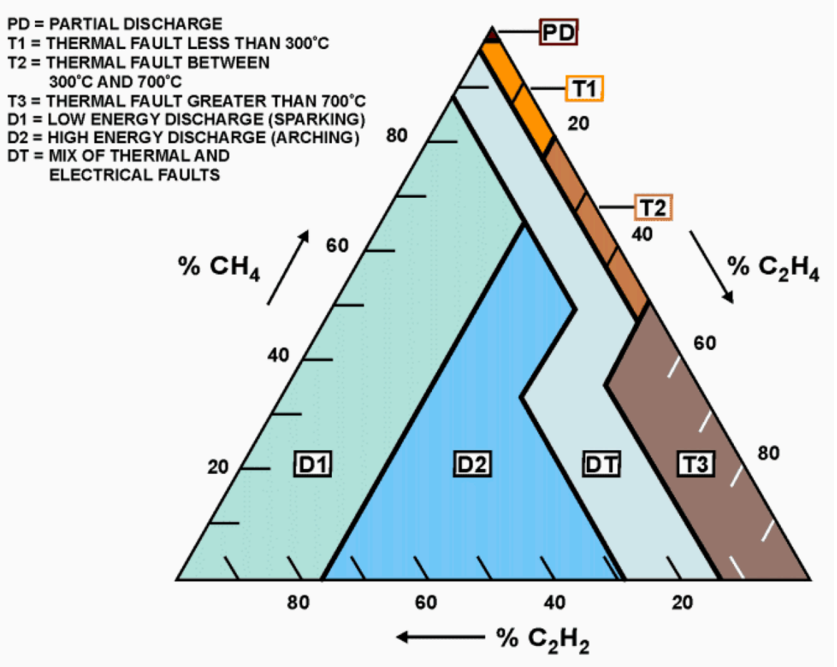
\includegraphics[width=0.7\textwidth]{figuras/Triangulo Duval.png}
\caption{Triângulo 1 de Duval para interpretação de gases dissolvidos em óleo mineral.}
\label{fig:Triangulo_Duval}
\fonte{Adaptado de \citeonline{ali2023}.}
\end{figure}

A área do triângulo é particionada em sete regiões correspondentes a diferentes mecanismos de falha:
descargas parciais (PD), delimitadas pela região com $\% \text{CH}_4 \ge 98\%$;
descargas de baixa energia (D1), definidas por $\% \text{C}_2\text{H}_2 > 13\%$ e $\% \text{C}_2\text{H}_4 < 23\%$;
descargas de alta energia (D2), delimitadas por $\% \text{C}_2\text{H}_2 \ge 29\%$ e $\% \text{C}_2\text{H}_4 \ge 23\%$, e pela sub-região com $\% \text{C}_2\text{H}_2$ entre 13\% e 29\% com $\% \text{C}_2\text{H}_4 \ge 23\%$;
falhas térmicas inferiores a 300~$^\circ\text{C}$ (T1), condicionadas a $\% \text{CH}_4 < 98\%$, $\% \text{C}_2\text{H}_2 < 4\%$ e $\% \text{C}_2\text{H}_4 < 20\%$;
falhas térmicas entre 300~$^\circ\text{C}$ e 700~$^\circ\text{C}$ (T2), delimitadas por $\% \text{C}_2\text{H}_2 < 4\%$ e $20\% \le \% \text{C}_2\text{H}_4 < 50\%$;
falhas térmicas superiores a 700~$^\circ\text{C}$ (T3), caracterizadas por $\% \text{C}_2\text{H}_2 < 15\%$ e $\% \text{C}_2\text{H}_4 \ge 50\%$;
e a zona de transição térmica e elétrica combinada (DT), delimitada por $\% \text{C}_2\text{H}_2$ entre 4\% e 13\% com $\% \text{C}_2\text{H}_4 \ge 20\%$ e $\% \text{C}_2\text{H}_4 < 50\%$.

A principal limitação do Triângulo 1 de Duval é a inexistência de uma região destinada à operação normal. Dessa forma, qualquer amostra projetada sobre o gráfico é classificada em alguma categoria de falha, podendo gerar falsos positivos em transformadores saudáveis que apresentem apenas taxas normais de gaseificação basal. Além disso, amostras localizadas muito próximas às linhas de fronteira sofrem com a sensibilidade a pequenas incertezas de medição, em que pequenas variações nas concentrações podem alterar a classe atribuída.

\subsection{Método das Razões da IEC 60599}\label{sec:razoes_iec}

O método analítico estabelecido pela norma IEC 60599 \cite{iec60599_2022} fundamenta-se no cálculo de três razões entre as concentrações dos gases dissolvidos:

\begin{equation}\label{eq:razoes_iec}
r_1 = \frac{[\text{C}_2\text{H}_2]}{[\text{C}_2\text{H}_4]}, \quad
r_2 = \frac{[\text{CH}_4]}{[\text{H}_2]}, \quad
r_3 = \frac{[\text{C}_2\text{H}_4]}{[\text{C}_2\text{H}_6]}
\end{equation}

A relação $r_1$ avalia a presença de acetileno em relação ao etileno, permitindo distinguir centelhamentos elétricos de sobreaquecimentos térmicos puros. A relação $r_2$ compara o metano com o hidrogênio, auxiliando na identificação do regime térmico de descargas ou aquecimentos iniciais. A relação $r_3$ confronta hidrocarbonetos insaturados com saturados, oferecendo sensibilidade direta à temperatura de degradação do óleo.

A norma estabelece intervalos discretos de valores para cada uma das razões, associando suas combinações aos tipos clássicos de falha. As descargas parciais (PD) exigem $r_1 < 0,1$, $r_2 < 0,1$ e $r_3 < 0,2$. As descargas de baixa energia (D1) requerem $r_1 > 1$, $0,1 \le r_2 \le 0,5$ e $r_3 > 1$, enquanto as descargas de alta energia (D2) são caracterizadas por $0,6 \le r_1 \le 2,5$, $0,1 \le r_2 \le 1$ e $r_3 > 2$. Para as falhas térmicas, a degradação de baixa temperatura inferior a 300~$^\circ\text{C}$ (T1) demanda $r_1 < 0,1$, $r_2 > 1$ e $r_3 < 1$. A faixa intermediária entre 300~$^\circ\text{C}$ e 700~$^\circ\text{C}$ (T2) requer $r_1 < 0,1$, $r_2 > 1$ e $1 \le r_3 \le 4$, enquanto as falhas de alta temperatura superiores a 700~$^\circ\text{C}$ (T3) exigem $r_1 < 0,2$, $r_2 > 1$ e $r_3 > 4$.

Caso a combinação de razões $(r_1, r_2, r_3)$ não corresponda a nenhum dos padrões catalogados na tabela da norma, o diagnóstico é classificado como Não Determinado (ND). Em dados de campo, a proporção de laudos indeterminados costuma ser considerável, principalmente em transformadores com falhas múltiplas combinadas ou ruídos de medição, o que limita a eficácia do método quando utilizado de maneira isolada. Assim como no Triângulo de Duval, a norma IEC 60599 não possui uma combinação específica para indicar condição normal de operação, exigindo que o diagnóstico por razões seja aplicado apenas após as concentrações ultrapassarem os limites típicos de atenção estabelecidos para a frota.

\section{Algoritmos de Aprendizado de Máquina Aplicados à DGA}\label{sec:algoritmos_ml}

Diante das limitações das abordagens normativas tradicionais, técnicas de aprendizado de máquina têm sido aplicadas para aprender fronteiras de decisão não lineares a partir de bancos de dados históricos de cromatografia.

\subsection{Panorama e Classificadores Clássicos}\label{sec:panorama_classificadores}

A Tabela~\ref{tab:algoritmos} apresenta um panorama comparativo das principais famílias de algoritmos avaliadas na literatura de diagnóstico em transformadores, destacando referências representativas, principais vantagens e limitações para a aplicação em DGA.

\renewcommand{\arraystretch}{1.4}

\begin{longtable}{
>{\RaggedRight\arraybackslash}p{2.6cm}
>{\RaggedRight\arraybackslash}p{2.2cm}
>{\RaggedRight\arraybackslash}p{3.6cm}
>{\RaggedRight\arraybackslash}p{3.8cm}
}

\caption{Comparação entre algoritmos de aprendizado de máquina aplicados à DGA}
\label{tab:algoritmos} \\

\hline
\textbf{Algoritmo} & \textbf{Referência em DGA} & \textbf{Vantagem principal} & \textbf{Limitação para este problema} \\
\hline
\endfirsthead

\multicolumn{4}{c}{\tablename\ \thetable{} -- continuação} \\
\hline
\textbf{Algoritmo} & \textbf{Referência em DGA} & \textbf{Vantagem principal} & \textbf{Limitação para este problema} \\
\hline
\endhead

\hline
\multicolumn{4}{r}{\textit{Continua na próxima página}} \\
\endfoot

\hline
\multicolumn{4}{p{\dimexpr\textwidth-2\tabcolsep\relax}}{\footnotesize Fonte: elaborado pelo autor com base em \citeonline{ali2023}, \citeonline{alsakini2025}, \citeonline{wu2021}, \citeonline{zhu2023} e \citeonline{lecun1998gradient}.} \\
\multicolumn{4}{p{\dimexpr\textwidth-2\tabcolsep\relax}}{\footnotesize Nota: $\checkmark$ indica as técnicas adotadas na formulação experimental deste estudo.} \\
\endlastfoot

\multicolumn{4}{l}{\textit{Classificadores clássicos}} \\
\hline
SVM & Al-Sakini et al. (2025) & Maximização de margem de separação em alta dimensão & Dificuldade em classes sobrepostas e expansão multiclasse não nativa \\

KNN & Ali et al. (2023) & Simplicidade conceitual sem premissas distributivas & Sensibilidade a ruídos locais e custo computacional alto na predição \\

Árvore de Decisão & Ali et al. (2023) & Facilidade de interpretação e extração direta de regras & Instabilidade a pequenas perturbações e tendência a sobreajuste \\

Random Forest & Al-Sakini et al. (2025) & Redução de variância por combinação de árvores & Dificuldade de sintonia simultânea de atributos e hiperparâmetros \\

Naive Bayes & Ali et al. (2023) & Simplicidade de cálculo e treinamento rápido & Suposição irrealista de independência entre os gases \\
\hline

\multicolumn{4}{l}{\textit{Ensembles e boosting}} \\
\hline
\textbf{XGBoost} $\checkmark$ & Wu et al. (2021) & Regularização explícita e ponderação para dados desbalanceados & Necessidade de ajuste hiperparamétrico e ausência de memória temporal \\

LightGBM & -- & Eficiência em bases volumosas por expansão foliar & Risco de sobreajuste em conjuntos com poucas centenas de amostras \\
\hline

\multicolumn{4}{l}{\textit{Redes neurais}} \\
\hline
MLP & Ali et al. (2023) & Capacidade de aproximação de funções não lineares & Ausência de mecanismos para modelar sequências temporais \\

CNN & LeCun et al. (1998) & Extração hierárquica de correlações espaciais & Estrutura voltada a matrizes espaciais, pouco natural para tabelas de gases \\
\hline

\multicolumn{4}{l}{\textit{Modelos de séries temporais}} \\
\hline
ARIMA & Ali et al. (2023) & Modelo estatístico linear simples e bem fundamentado & Premissa de linearidade e dificuldade de modelagem multivariada \\

\textbf{LSTM} $\checkmark$ & Katser et al. (2022) & Captura de dependências temporais longas por mecanismos de portas & Custo de treino superior e necessidade de séries regulares \\

Transformer & Zhu et al. (2023) & Mecanismos de atenção em horizontes longos & Exigência de grandes volumes de dados, indisponíveis em DGA aberta \\
\hline

\multicolumn{4}{l}{\textit{Otimização evolutiva}} \\
\hline
AG padrão & Ali et al. (2023) & Busca estocástica global sem necessidade de derivadas & Risco de convergência prematura em problemas multimodais \\

\textbf{IGA} $\checkmark$ & Wu et al. (2021) & Cruzamento adaptativo, operadores mistos e elitismo & Custo computacional elevado pela validação cruzada iterativa \\

Otimização Bayesiana & -- & Amostragem baseada em processos gaussianos & Menor flexibilidade para otimizar conjuntamente variáveis binárias e contínuas \\

\end{longtable}

Entre os classificadores clássicos, as Máquinas de Vetores de Suporte (SVM) apresentam bom desempenho na separação de classes em espaços mapeados por funções de base radial, mas têm dificuldade em regiões com forte sobreposição entre classes vizinhas, como as falhas térmicas T2 e T3 \cite{alsakini2025}. Modelos baseados em vizinhos mais próximos (KNN) e árvores de decisão simples sofrem com a presença de ruído e alta variância. O Random Forest ameniza essa variância ao combinar múltiplas árvores independentes por amostragem com reposição (\textit{bagging}), contudo não dispõe de um mecanismo integrado para selecionar atributos e otimizar hiperparâmetros de forma conjunta. Por fim, o Naive Bayes, embora simples para estabelecer uma linha de base, assume que as variáveis preditoras são independentes entre si, premissa que não reflete a realidade físico-química da DGA, na qual os gases são gerados por processos de degradação térmica e elétrica inter-relacionados \cite{ali2023}.

\subsection{Ensembles de Árvores e o Algoritmo XGBoost}\label{sec:xgboost}

Os métodos de \textit{gradient boosting} constroem modelos preditivos por meio da combinação sequencial aditiva de estimadores fracos, tipicamente árvores de decisão de profundidade moderada \cite{friedman2001}. A cada iteração $k$, uma nova árvore $f_k(x)$ é ajustada para estimar o gradiente negativo da função de perda em relação à predição atual, reduzindo progressivamente os erros residuais, conforme ilustrado na Figura~\ref{fig:xgboost}.

\begin{figure}[htbp]
\centering
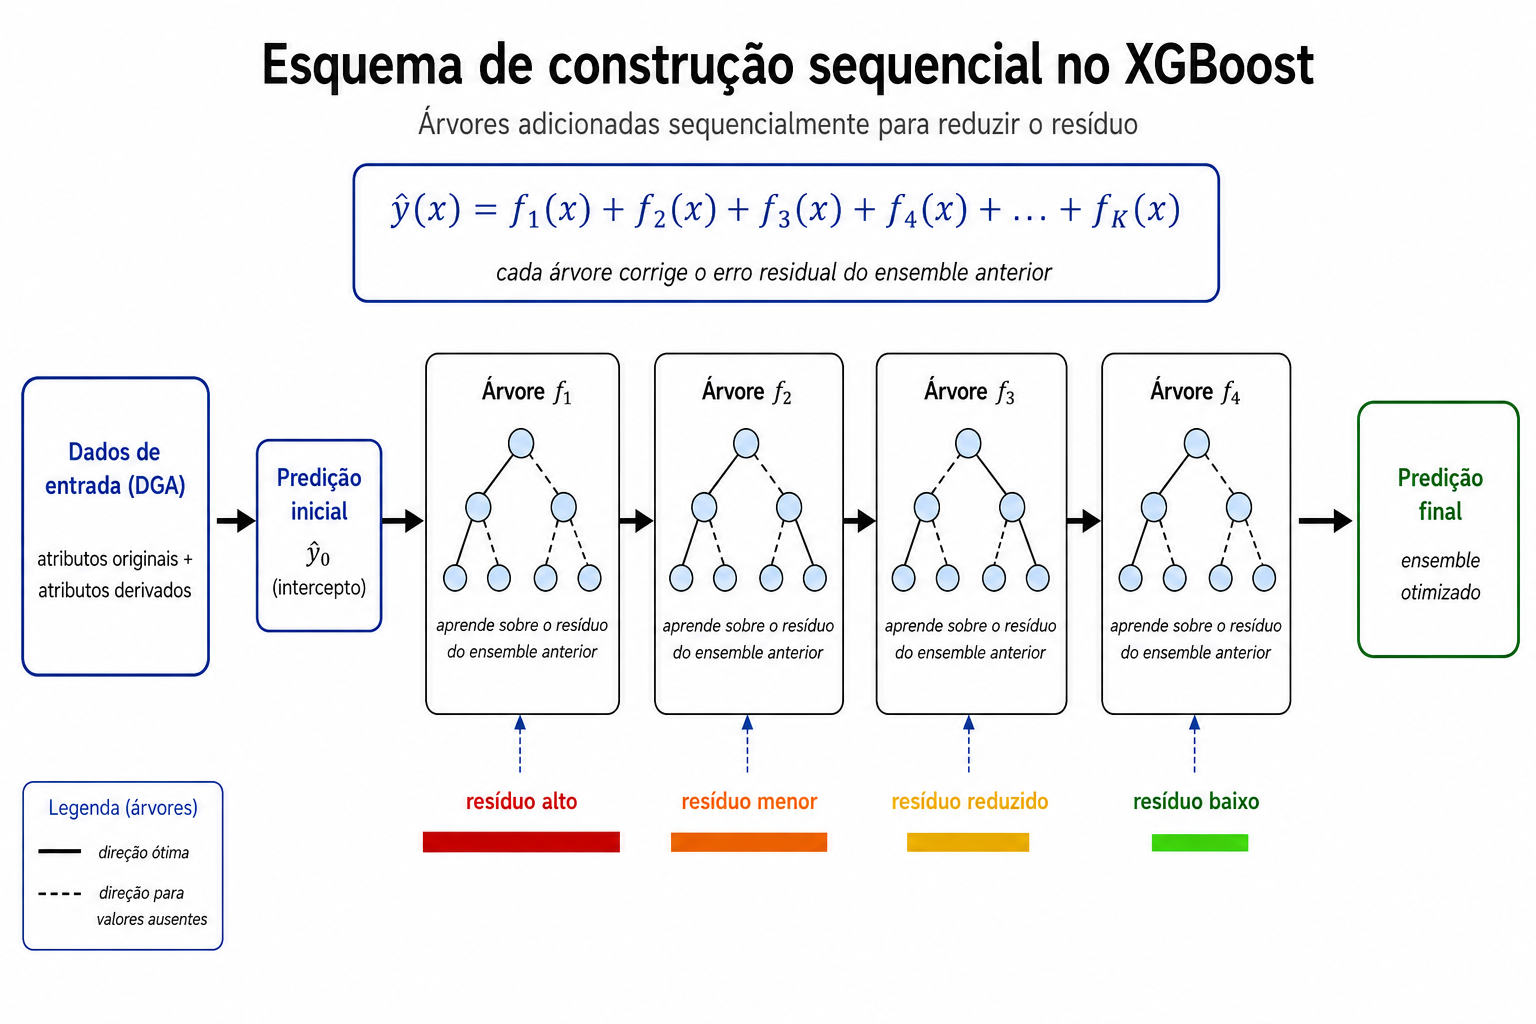
\includegraphics[width=0.8\textwidth]{figuras/xgboost.png}
\caption{Processo iterativo de minimização de resíduos em ensembles de gradient boosting.}
\label{fig:xgboost}
\fonte{Elaborado pelo autor.}
\end{figure}

A predição final de uma amostra $x$ após a inclusão de $K$ árvores é obtida pela soma das contribuições de cada estimador:

\begin{equation}\label{eq:xgboost_pred}
\hat{y}(x) = \sum_{k=1}^{K} f_k(x), \quad f_k \in \mathcal{F}
\end{equation}

O algoritmo XGBoost (\textit{Extreme Gradient Boosting}) introduz formulações que melhoram a estabilidade, a precisão e a velocidade de convergência em relação ao boosting tradicional \cite{chen2016_xgboost}. A função objetivo minimizada na iteração $t$ incorpora termos explícitos de regularização sobre a estrutura das árvores:

\begin{equation}\label{eq:xgboost_obj}
\mathcal{L}^{(t)} = \sum_{i=1}^{N} l\left(y_i, \hat{y}_i^{(t-1)} + f_t(x_i)\right) + \sum_{k=1}^{t} \Omega(f_k)
\end{equation}

Em que $l$ representa a função de perda diferenciável e $\Omega(f)$ define o termo de regularização da árvore, expresso por:

\begin{equation}\label{eq:xgboost_omega}
\Omega(f) = \gamma T_L + \frac{1}{2} \lambda_{\text{reg}} \sum_{j=1}^{T_L} w_j^2 + \alpha_{\text{reg}} \sum_{j=1}^{T_L} |w_j|
\end{equation}

Nessa expressão, $T_L$ denota o número de folhas da árvore, $w_j$ é o peso associado à folha $j$, $\gamma$ representa o custo de complexidade para a criação de novas folhas e os parâmetros $\lambda_{\text{reg}}$ e $\alpha_{\text{reg}}$ correspondem aos termos de regularização $L_2$ e $L_1$, respectivamente. A expansão de Taylor em segunda ordem da função de perda permite calcular de forma analítica o ganho de divisão dos nós e os pesos ótimos das folhas, garantindo convergência eficiente e controle contra o sobreajuste.

Para lidar com o desbalanceamento característico de bases de dados de DGA, o XGBoost suporta a atribuição de pesos diferenciados por instância (\texttt{sample\_weight}), permitindo ponderar a contribuição das amostras na função de perda de forma inversamente proporcional à frequência de cada classe.

\subsection{Redes Neurais Recorrentes e Modelagem Temporal}\label{sec:redes_lstm}

Redes neurais artificiais tradicionais assumem independência entre as amostras de entrada, não sendo capazes de processar ordenamento temporal contínuo. As Redes Neurais Recorrentes (RNN) superam essa restrição ao incorporar conexões de realimentação que mantêm um vetor de estado oculto $h_t$, atualizado a cada passo de tempo $t$ a partir da entrada atual $x_t$ e do estado anterior $h_{t-1}$:

\begin{equation}\label{eq:rnn_basica}
h_t = \tanh\left(W_x x_t + W_h h_{t-1} + b\right)
\end{equation}

No treinamento de RNNs convencionais pelo algoritmo de retropropagação no tempo (\textit{Backpropagation Through Time}, BPTT), a multiplicação sucessiva de matrizes de pesos ao longo de muitos passos temporais tende a provocar o desaparecimento do gradiente (\textit{vanishing gradient}), reduzindo a capacidade do modelo em capturar dependências de longo prazo \cite{hochreiter1997long}.

A arquitetura \textit{Long Short-Term Memory} (LSTM) soluciona essa dificuldade por meio de uma célula de memória dedicada, regulada por mecanismos de portas (\textit{gates}) que controlam o fluxo de informação com conexões aditivas diretas \cite{hochreiter1997long}. O funcionamento da célula LSTM, detalhado na Figura~\ref{fig:celula_lstm}, é descrito pelo seguinte conjunto de equações:

\begin{equation}\label{eq:lstm_forget}
f_t = \sigma\left(W_f [h_{t-1}, x_t] + b_f\right)
\end{equation}

\begin{equation}\label{eq:lstm_input}
i_t = \sigma\left(W_i [h_{t-1}, x_t] + b_i\right)
\end{equation}

\begin{equation}\label{eq:lstm_candidate}
\tilde{C}_t = \tanh\left(W_c [h_{t-1}, x_t] + b_c\right)
\end{equation}

\begin{equation}\label{eq:lstm_cell}
C_t = f_t \odot C_{t-1} + i_t \odot \tilde{C}_t
\end{equation}

\begin{equation}\label{eq:lstm_output}
o_t = \sigma\left(W_o [h_{t-1}, x_t] + b_o\right)
\end{equation}

\begin{equation}\label{eq:lstm_hidden}
h_t = o_t \odot \tanh(C_t)
\end{equation}

Nas Equações~(\ref{eq:lstm_forget}) a (\ref{eq:lstm_hidden}), $\sigma$ denota a função sigmoide, $\odot$ representa o produto elemento a elemento de Hadamard, $f_t$ é a porta de esquecimento que modula o descarte de informações da célula anterior $C_{t-1}$, $i_t$ é a porta de entrada que regula a absorção do novo candidato $\tilde{C}_t$, $C_t$ é o estado interno da célula e $o_t$ é a porta de saída que determina a parcela de informação exposta no estado oculto $h_t$.

\begin{figure}[htbp]
\centering
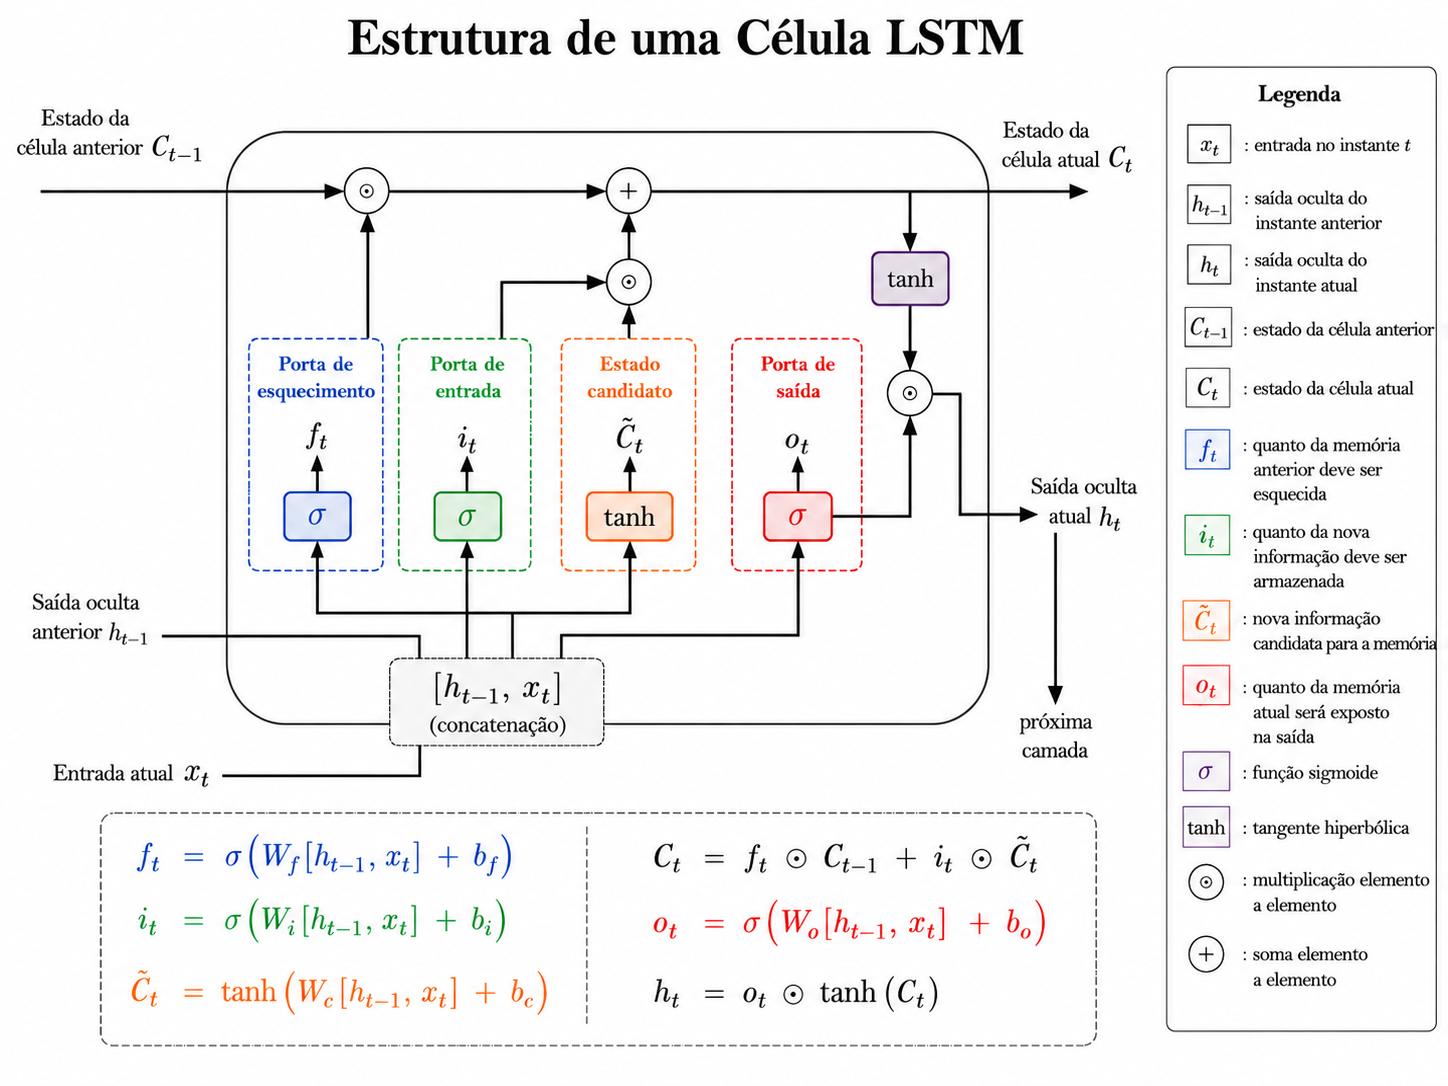
\includegraphics[width=0.75\textwidth]{figuras/celula_lstm.png}
\caption{Arquitetura estrutural da célula de memória recorrente LSTM.}
\label{fig:celula_lstm}
\fonte{Elaborado pelo autor com base em \citeonline{hochreiter1997long}.}
\end{figure}

Para modelar dinâmicas temporais complexas em séries temporais de gases, emprega-se a LSTM empilhada (\textit{Stacked LSTM}), que conecta múltiplas camadas recorrentes em série, conforme mostrado na Figura~\ref{fig:lstm_stacked}. Nesse formato, as saídas ocultas da primeira camada servem como sequência de entrada para a camada subsequente, permitindo capturar padrões de evolução das concentrações gasosas ao longo do tempo.

\begin{figure}[htbp]
\centering
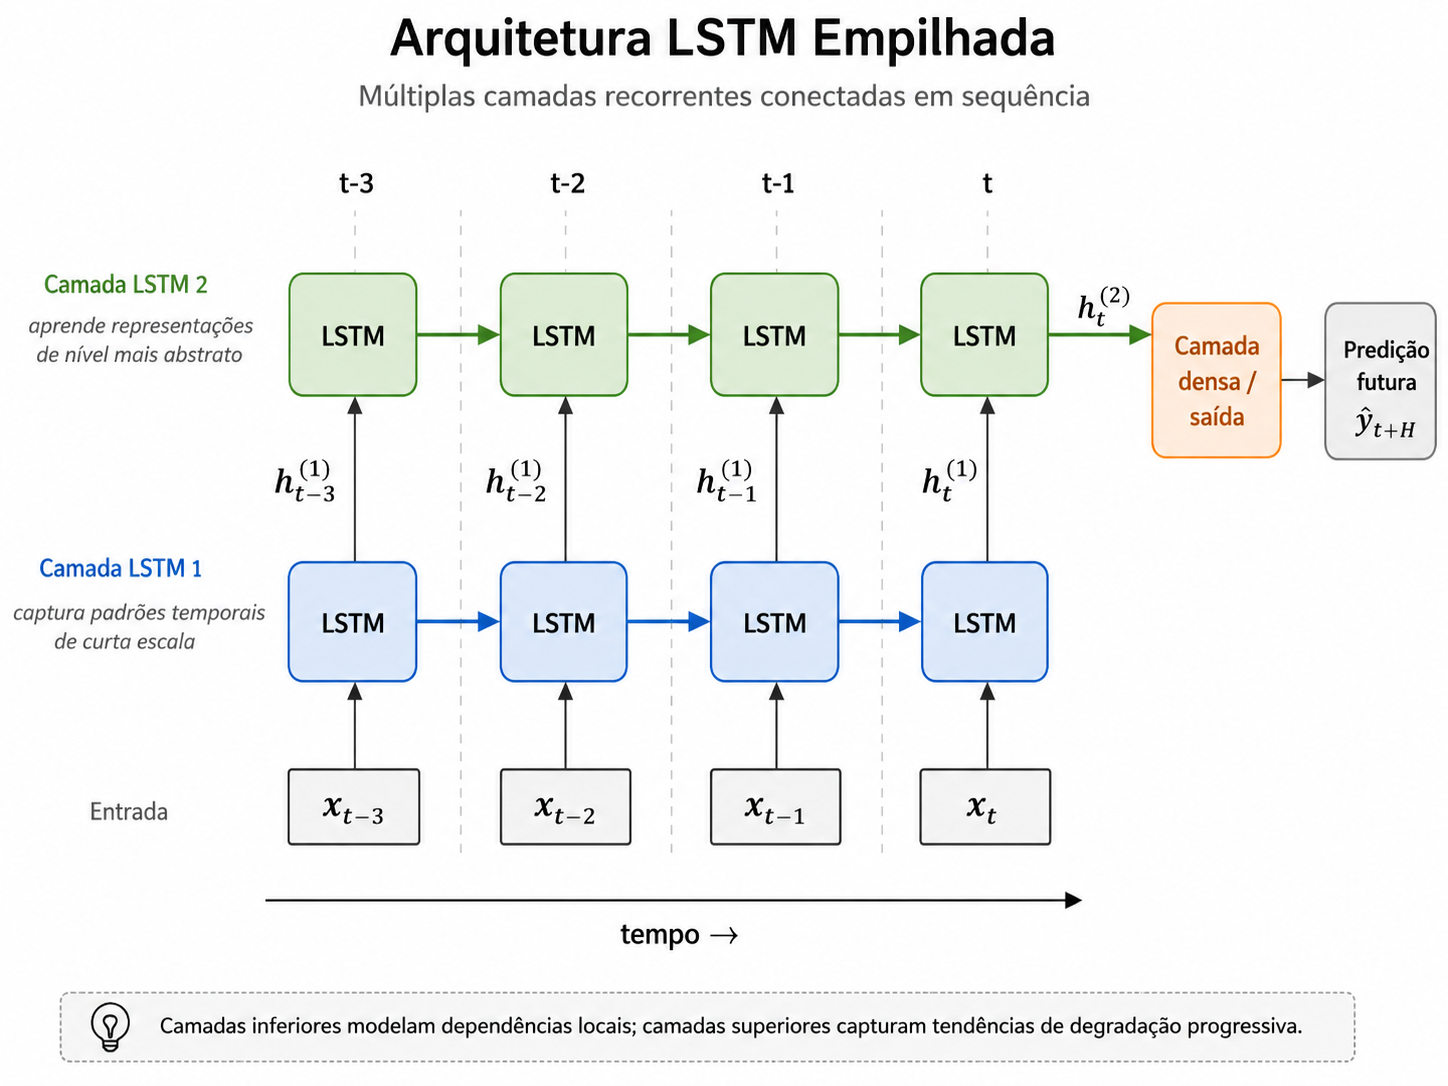
\includegraphics[width=0.75\textwidth]{figuras/LSTM_stacked.png}
\caption{Topologia de rede neural recorrente LSTM empilhada para modelagem temporal.}
\label{fig:lstm_stacked}
\fonte{Elaborado pelo autor.}
\end{figure}

\subsection{Otimização Evolutiva por Algoritmo Genético Melhorado (IGA)}\label{sec:iga}

O ajuste de um classificador XGBoost envolve uma escolha simultânea entre os atributos de entrada mais relevantes e a calibração de seus hiperparâmetros de complexidade e regularização. Os Algoritmos Genéticos (AG) constituem uma técnica de busca estocástica global inspirada nos princípios da evolução natural e da seleção dos indivíduos mais aptos \cite{ali2023}. O procedimento mantém uma população de soluções candidatas ao longo de sucessivas gerações, aplicando operadores de seleção por aptidão, recombinação por cruzamento (\textit{crossover}) e mutação.

Em matrizes de dados de DGA, o algoritmo genético clássico pode sofrer com convergência prematura em mínimos locais. O Algoritmo Genético Melhorado (IGA) contorna essa limitação incorporando mecanismos específicos de diversidade e conservação, conforme ilustrado na Figura~\ref{fig:IGA} \cite{wu2021}.

\begin{figure}[htbp]
\centering
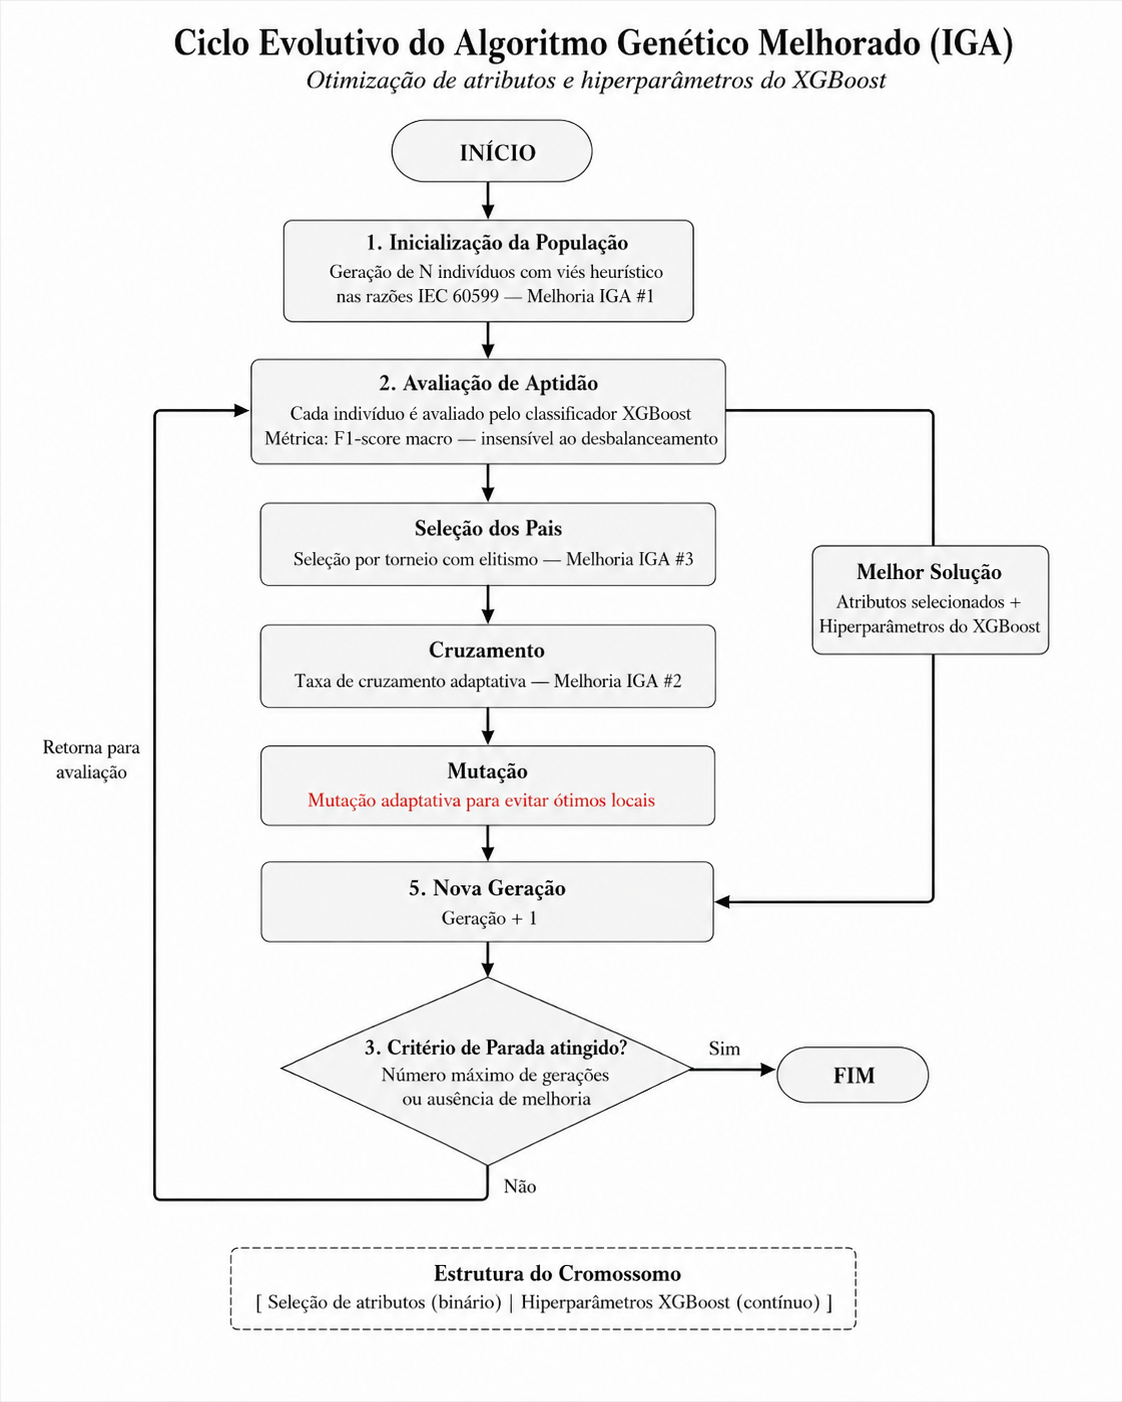
\includegraphics[width=0.55\textwidth]{figuras/IGA.png}
\caption{Fluxo operacional do Algoritmo Genético Melhorado para busca conjunta.}
\label{fig:IGA}
\fonte{Adaptado de \citeonline{wu2021}.}
\end{figure}

No IGA, cada indivíduo é estruturado por um cromossomo bipartido: uma máscara binária (que define quais variáveis são utilizadas) e um vetor de números reais (correspondente aos hiperparâmetros contínuos do XGBoost). Na etapa de recombinação, aplica-se cruzamento uniforme sobre a máscara binária e cruzamento linear adaptativo (\textit{Blend Crossover}, BLX-$\alpha$) sobre os genes contínuos, associados a perturbações gaussianas para mutação contínua e inversão probabilística de bits para a parte discreta. A preservação por elitismo garante que as melhores soluções encontradas sejam repassadas diretamente para a geração seguinte, guiando a busca para configurações de alta precisão e menor complexidade.

\section{Interpretabilidade em Aprendizado de Máquina (XAI)}\label{sec:xai_shap}

Na aplicação de aprendizado de máquina em sistemas críticos como redes elétricas de alta tensão, a compreensão dos fatores que determinam cada diagnóstico é essencial para que os resultados sejam aceitos e validados por equipes de engenharia. A área de inteligência artificial explicável (\textit{Explainable Artificial Intelligence}, XAI) fornece fundamentos matemáticos para quantificar a contribuição individual de cada variável de DGA nas predições geradas pelos modelos.

\subsection{Teoria dos Jogos Cooperativos e Valores de Shapley}\label{sec:valores_shapley}

A formulação matemática dos valores de Shapley origina-se na teoria dos jogos cooperativos com utilidade transferível \cite{shapley1953}. Define-se um jogo cooperativo pelo par $(F, v)$, no qual $F = \{1, 2, \dots, M\}$ representa o conjunto de jogadores (atributos preditores) e $v: 2^F \to \mathbb{R}$ é a função característica que associa um ganho real a cada subconjunto possível $S \subseteq F$, assumindo-se convencionalmente $v(\emptyset) = 0$.

O valor de Shapley $\phi_i(v)$ atribui a cada atributo $i$ uma parcela justa do resultado global da coalizão completa $v(F)$, ponderando a contribuição marginal média do atributo sobre todas as ordens possíveis de formação dos grupos:

\begin{equation}\label{eq:shapley_formula}
\phi_i(v) = \sum_{S \subseteq F \setminus \{i\}} \frac{|S|! \, (|F| - |S| - 1)!}{|F|!} \left[ v(S \cup \{i\}) - v(S) \right]
\end{equation}

A formulação da Equação~(\ref{eq:shapley_formula}) é a única partição de contribuição que satisfaz simultaneamente quatro propriedades fundamentais \cite{lundberg2017}:

\begin{itemize}
    \item \textbf{Eficiência}: a soma das contribuições distribuídas a todos os atributos reproduz exatamente a diferença entre a saída do modelo para a amostra e o valor esperado médio, satisfazendo $\sum_{i \in F} \phi_i(v) = v(F) - v(\emptyset)$;
    \item \textbf{Simetria}: se dois atributos exercem contribuições marginais idênticas para qualquer combinação intermediária, de modo que $v(S \cup \{i\}) = v(S \cup \{j\})$ para todo $S \subseteq F \setminus \{i, j\}$, seus valores de Shapley serão iguais, $\phi_i(v) = \phi_j(v)$;
    \item \textbf{Atributo nulo}: se uma variável não altera o ganho de nenhum subconjunto, satisfazendo $v(S \cup \{i\}) = v(S)$ para todo $S \subseteq F \setminus \{i\}$, sua contribuição associada é nula, $\phi_i(v) = 0$;
    \item \textbf{Aditividade}: para dois modelos combinados linearmente, a atribuição de crédito satisfaz $\phi_i(u + v) = \phi_i(u) + \phi_i(v)$.
\end{itemize}

\subsection{O Algoritmo TreeSHAP e Decomposição de Contribuições}\label{sec:treeshap}

O cálculo direto da Equação~(\ref{eq:shapley_formula}) possui complexidade temporal exponencial $O(M 2^M)$, tornando-se inviável para modelos com muitos atributos. Para viabilizar esse cálculo em conjuntos de árvores de decisão, \citeonline{lundberg2020} propuseram o algoritmo TreeSHAP, que calcula os valores exatos de Shapley em tempo polinomial $O(T L D^2)$, onde $T$ é o número de árvores, $L$ é o número máximo de folhas e $D$ representa a profundidade máxima das árvores.

Em classificadores multiclasse como o XGBoost, o TreeSHAP calcula as contribuições diretamente no espaço linear das margens de decisão (\textit{log-odds}) antes da aplicação da função softmax (\texttt{pred\_contribs}). Para cada classe diagnóstica $c$, a pontuação $f_c(x)$ da amostra $x$ é decomposta de forma exata:

\begin{equation}\label{eq:treeshap_add}
f_c(x) = \phi_{0,c} + \sum_{i=1}^{M} \phi_{i,c}(x)
\end{equation}

Em que $\phi_{0,c} = \mathbb{E}[f_c(X)]$ denota o valor médio basal da classe $c$ sobre a base de treinamento, e $\phi_{i,c}(x)$ corresponde à contribuição aditiva individual da variável $i$. Vale destacar que o valor de Shapley indica quanto a variável contribui para aumentar ($\phi > 0$) ou diminuir ($\phi < 0$) a probabilidade daquela classe específica, enquanto a classe final prevista corresponde àquela com maior escore conjunto via $\arg\max_c f_c(x)$.

Para isolar as dependências entre pares de variáveis, o algoritmo também calcula a matriz de interação de Lundberg (\texttt{pred\_interactions}) baseada no índice de interação de Shapley \cite{lundberg2020}:

\begin{equation}\label{eq:shapley_interaction}
\phi_{i,j}(x) = \sum_{S \subseteq F \setminus \{i, j\}} \frac{|S|! \, (|F| - |S| - 2)!}{2 \, (|F| - 1)!} \left[ v(S \cup \{i, j\}) - v(S \cup \{i\}) - v(S \cup \{j\}) + v(S) \right]
\end{equation}

Para $i \ne j$, $\phi_{i,j}(x)$ mede a interação de segunda ordem entre os atributos $i$ e $j$. A diagonal principal da matriz permite isolar o efeito principal univariado de cada variável $\phi_{i,i}(x)$:

\begin{equation}\label{eq:main_effect}
\phi_{i,i}(x) = \phi_i(x) - \sum_{j \neq i} \phi_{i,j}(x)
\end{equation}

Ao relacionar o efeito principal $\phi_{i,i}(x)$ com o valor físico real da variável (em ppm ou em percentual relativo), é possível identificar o ponto em que a contribuição transita de negativa para positiva ($\phi_{i,i} = 0$), permitindo comparar os critérios aprendidos pelo XGBoost com os limiares práticos das normas da IEC e do Triângulo de Duval.

\section{Trabalhos Relacionados}\label{sec:trabalhos_relacionados}

O diagnóstico preditivo de falhas em transformadores por meio de DGA tem evoluído de métodos gráficos tradicionais para técnicas baseadas em modelos computacionais de aprendizado de máquina. A Tabela~\ref{tab:comparacao_trabalhos} sintetiza os principais estudos representativos da literatura recente, comparando suas abordagens, dados utilizados, principais vantagens e limitações observadas.

\begin{table}[htbp]
\centering
\caption{Comparação entre trabalhos relacionados e o escopo investigado neste estudo.}
\label{tab:comparacao_trabalhos}
\resizebox{\textwidth}{!}{
\begin{tabular}{|p{3.0cm}|p{3.2cm}|p{2.5cm}|p{4.0cm}|p{4.2cm}|}
\hline
\textbf{Trabalho} & \textbf{Abordagem} & \textbf{Tipo} & \textbf{Vantagens} & \textbf{Limitações} \\
\hline
Wu et al. (2021) & IGA + XGBoost & Classificação & Otimização simultânea de atributos e hiperparâmetros com acurácia elevada & Diagnóstico puramente estático, ausência de avaliação temporal e métricas globais sem detalhamento por classe \\
\hline
Wang et al. (2023) & LSTM + Classificadores & Previsão + Classificação & Modelagem da evolução temporal de gases para antecipação de falhas & Classificação desacoplada da etapa preditiva e uso de base de dados restrita \\
\hline
Ali et al. (2023) & Métodos Tradicionais e Revisão de ML & Revisão & Levantamento abrangente de normas de DGA e métodos inteligentes & Ausência de validação experimental direta e sem modelo computacional proposto \\
\hline
Al-Sakini et al. (2025) & Aprendizado de Máquina Supervisionado & Classificação & Validação empírica sobre registros laboratoriais reais de transformadores & Abordagem exclusivamente estática e sensibilidade a sobreposição de classes \\
\hline
Tightiz et al. (2020) & ANFIS + Regras de Associação & Classificação & Integração de inferência neuro-fuzzy com regras de diagnóstico & Ajuste complexo de muitas regras e ausência de componente temporal \\
\hline
Zhu et al. (2023) & Transformers em Séries Temporais & Previsão & Atenção em dependências temporais em sistemas de potência & Custo computacional elevado e demanda de grande volume de dados \\
\hline
\textbf{Abordagem deste Trabalho} & LSTM Empilhada + IGA-XGBoost + TreeSHAP & Híbrido em Dois Eixos & Avaliação do impacto de previsões temporais, seleção de atributos por IGA e interpretação física com TreeSHAP & Separação em dois eixos devido às características distintas das bases de dados públicas disponíveis \\
\hline
\end{tabular}
}
\fonte{Elaborado pelo autor.}
\end{table}

A análise crítica dos estudos da literatura indica que os trabalhos costumam apresentar lacunas metodológicas importantes. O estudo de \citeonline{wu2021} obteve bons resultados ao combinar seleção de variáveis e ajuste de hiperparâmetros por IGA com o XGBoost, reportando acurácias superiores a 99\% em dados normativos. No entanto, o trabalho avaliou apenas dados estáticos pontuais, sem considerar séries temporais, além de reportar métricas globais de acurácia que podem mascarar o desempenho em classes minoritárias.

Por outro lado, o trabalho de \citeonline{wang2023} focou na modelagem temporal com redes LSTM para estimar concentrações futuras de gases. Contudo, a etapa de previsão foi avaliada de forma desvinculada do classificador final, sem um teste controlado para verificar se a inclusão das estimativas futuras realmente melhorava a precisão do diagnóstico em relação aos gases já conhecidos no momento presente. Além disso, a base de dados utilizada era de acesso restrito, dificultando comparações diretas.

Por sua vez, \citeonline{alsakini2025} testaram diversos modelos de aprendizado supervisionado em dados laboratoriais reais, confirmando que ensembles de árvores superam modelos simples em conjuntos com ruído, mas também se limitaram a diagnósticos pontuais estáticos. Já as revisões conduzidas por \citeonline{ali2023} apontam que as principais carências da área incluem a falta de protocolos estatísticos para lidar com o desbalanceamento real das classes, a escassez de modelos que combinem dinâmicas temporais com classificadores otimizados e a ausência de análises que interpretem fisicamente as decisões dos algoritmos à luz das normas técnicas.

Por fim, o uso de arquiteturas Transformer em séries temporais de transformadores, explorado por \citeonline{zhu2023}, confirma a utilidade dos mecanismos de autoatenção para sequências longas, mas esbarra na exigência de grandes volumes de dados de treinamento, raramente disponíveis em bases públicas abertas de DGA.

Com base nesse panorama, este trabalho estrutura sua metodologia em dois eixos complementares: utiliza dados industriais saneados, testa de forma controlada o impacto de previsões temporais da LSTM acopladas ao XGBoost, emprega o algoritmo genético para selecionar subconjuntos enxutos de atributos e analisa as regras aprendidas pelo modelo com base em valores de Shapley, aproximando as decisões dos algoritmos dos critérios estabelecidos pelas normas técnicas de DGA.
